% Chapter 9: Latest Research and Breakthroughs (2023-2024)

\section{Latest Research}

% Section Introduction
\sectionintro{Latest Research}{\faRocket}{Cutting-edge developments in embeddings}

% Matryoshka Embeddings
\begin{conceptslide}{Matryoshka Embeddings: Adaptive Dimensionality}{4}
\textbf{One Model, Multiple Dimensions}

\begin{columns}
\column{0.5\textwidth}
\begin{conceptbox}{The Innovation}
Embeddings that work at multiple dimensions simultaneously:
\begin{itemize}
    \item Train once, use at any size
    \item First $k$ dimensions are meaningful for any $k$
    \item 2-16x efficiency gains
\end{itemize}
\end{conceptbox}

\textbf{How It Works:}
\begin{enumerate}
    \item Train with nested loss functions
    \item Each prefix is independently useful
    \item Dynamic truncation at inference
\end{enumerate}

\column{0.5\textwidth}
\begin{mathbox}
\textbf{Training Objective:}
$$\mathcal{L} = \sum_{d \in \{32, 64, 128, ..., 768\}} \alpha_d \mathcal{L}_d$$

where $\mathcal{L}_d$ uses only first $d$ dimensions
\end{mathbox}

\textbf{Performance:}
\begin{center}
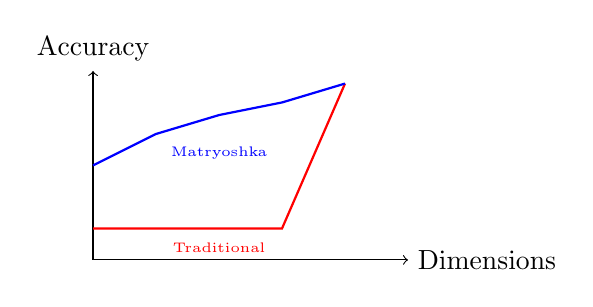
\begin{tikzpicture}[scale=0.8]
    \draw[->] (0,0) -- (5,0) node[right] {Dimensions};
    \draw[->] (0,0) -- (0,3) node[above] {Accuracy};
    
    % Traditional
    \draw[red,thick] (0,0.5) -- (1,0.5) -- (2,0.5) -- (3,0.5) -- (4,2.8);
    \node[red] at (2,0.2) {\tiny Traditional};
    
    % Matryoshka
    \draw[blue,thick] (0,1.5) -- (1,2) -- (2,2.3) -- (3,2.5) -- (4,2.8);
    \node[blue] at (2,1.7) {\tiny Matryoshka};
\end{tikzpicture}
\end{center}

\begin{trybox}
Use 32 dims for search, 768 for ranking!
\end{trybox}
\end{columns}
\end{conceptslide}

% RAG-Optimized Embeddings
\begin{conceptslide}{RAG-Optimized Embeddings}{4}
\textbf{Embeddings for Retrieval-Augmented Generation}

\begin{columns}
\column{0.5\textwidth}
\textbf{The Challenge:}
Traditional embeddings weren't designed for RAG:
\begin{itemize}
    \item Need both similarity AND informativeness
    \item Must handle query-document asymmetry
    \item Balance precision vs recall
\end{itemize}

\vspace{0.3cm}
\textbf{Recent Advances (2024):}
\begin{enumerate}
    \item \concept{Contriever}: Self-supervised RAG training
    \item \concept{E5-Mistral}: LLM-based embeddings
    \item \concept{BGE-M3}: Multi-lingual, multi-granular
\end{enumerate}

\column{0.5\textwidth}
\begin{insightbox}
RAG embeddings optimize for different objectives than semantic similarity alone!
\end{insightbox}

\textbf{Key Innovations:}
\begin{itemize}
    \item \iconAttention\ \textbf{Cross-Attention Training}: 
    Learn query-doc interactions
    
    \item \iconNetwork\ \textbf{Hard Negative Mining}:
    Distinguish subtle differences
    
    \item \iconOptimize\ \textbf{Multi-Task Learning}:
    Balance multiple objectives
\end{itemize}

\textbf{Benchmark Results:}
\begin{center}
\small
\begin{tabular}{lcc}
\toprule
Model & BEIR & MS MARCO \\
\midrule
BERT & 38.2 & 33.5 \\
Contriever & 42.1 & 35.8 \\
E5-Large & 45.6 & 38.9 \\
BGE-M3 & \textbf{47.2} & \textbf{40.1} \\
\bottomrule
\end{tabular}
\end{center}
\end{columns}
\end{conceptslide}

% Cross-Modal Embeddings
\begin{conceptslide}{Beyond Text: Cross-Modal Embeddings}{5}
\textbf{Unified Representation Across Modalities}

\begin{columns}
\column{0.6\textwidth}
\textbf{Recent Breakthroughs:}

\begin{enumerate}
    \item \concept{CLIP Evolution (2024)}
    \begin{itemize}
        \item SigLIP: Sigmoid loss for better training
        \item OpenCLIP: Scaled to 5B parameters
        \item MetaCLIP: Metadata-curated training
    \end{itemize}
    
    \item \concept{ImageBind (Meta, 2023)}
    \begin{itemize}
        \item 6 modalities in one space
        \item Text, Image, Audio, Video, Thermal, Depth
        \item Zero-shot cross-modal retrieval
    \end{itemize}
    
    \item \concept{BLIP-2 (2023)}
    \begin{itemize}
        \item Efficient vision-language pre-training
        \item Q-Former architecture
        \item 7B parameter performance with 54x fewer params
    \end{itemize}
\end{enumerate}

\column{0.4\textwidth}
\textbf{Unified Embedding Space:}
\begin{center}
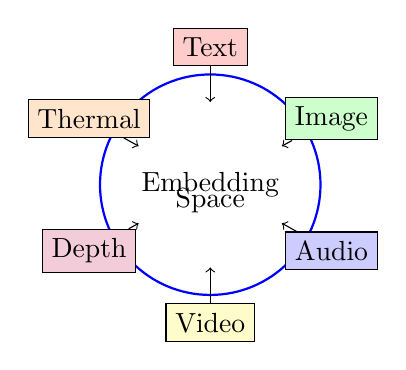
\begin{tikzpicture}[scale=0.7]
    % Central embedding space
    \draw[thick,blue] (0,0) circle (2);
    \node at (0,0) {Embedding};
    \node at (0,-0.3) {Space};
    
    % Modalities
    \node[draw,fill=red!20] (text) at (0,2.5) {Text};
    \node[draw,fill=green!20] (image) at (2.2,1.2) {Image};
    \node[draw,fill=blue!20] (audio) at (2.2,-1.2) {Audio};
    \node[draw,fill=yellow!20] (video) at (0,-2.5) {Video};
    \node[draw,fill=purple!20] (depth) at (-2.2,-1.2) {Depth};
    \node[draw,fill=orange!20] (thermal) at (-2.2,1.2) {Thermal};
    
    % Connections
    \draw[->] (text) -- (0,1.5);
    \draw[->] (image) -- (1.3,0.7);
    \draw[->] (audio) -- (1.3,-0.7);
    \draw[->] (video) -- (0,-1.5);
    \draw[->] (depth) -- (-1.3,-0.7);
    \draw[->] (thermal) -- (-1.3,0.7);
\end{tikzpicture}
\end{center}

\begin{warningbox}
Cross-modal alignment is still imperfect - expect 10-20\% performance drop
\end{warningbox}
\end{columns}
\end{conceptslide}

% Efficient Embedding Techniques
\begin{conceptslide}{Efficiency Revolution: Faster, Smaller, Better}{3}
\textbf{Making Embeddings Practical at Scale}

\begin{columns}
\column{0.5\textwidth}
\textbf{1. Quantization Advances:}
\begin{itemize}
    \item \concept{Binary Embeddings}: 1-bit per dimension
    \item \concept{Product Quantization}: 32x compression
    \item \concept{Learned Quantization}: Task-specific compression
\end{itemize}

\textbf{2. Distillation Techniques:}
\begin{itemize}
    \item Teacher-Student with only 10\% size
    \item Progressive distillation stages
    \item Task-specific fine-tuning
\end{itemize}

\textbf{3. Sparse Embeddings:}
\begin{itemize}
    \item SPLADE v2: Learned sparse representations
    \item ColBERT v2: Late interaction efficiency
    \item Hybrid dense-sparse approaches
\end{itemize}

\column{0.5\textwidth}
\textbf{Performance vs Efficiency Trade-offs:}

\begin{center}
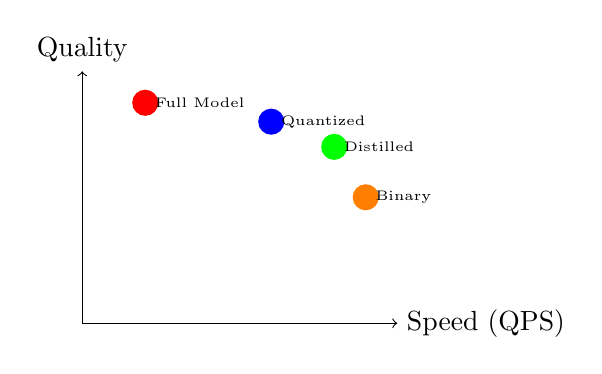
\begin{tikzpicture}[scale=0.8]
    \draw[->] (0,0) -- (5,0) node[right] {Speed (QPS)};
    \draw[->] (0,0) -- (0,4) node[above] {Quality};
    
    % Plot points
    \node[circle,fill=red] (full) at (1,3.5) {};
    \node[right] at (full) {\tiny Full Model};
    
    \node[circle,fill=blue] (quant) at (3,3.2) {};
    \node[right] at (quant) {\tiny Quantized};
    
    \node[circle,fill=green] (distill) at (4,2.8) {};
    \node[right] at (distill) {\tiny Distilled};
    
    \node[circle,fill=orange] (binary) at (4.5,2) {};
    \node[right] at (binary) {\tiny Binary};
\end{tikzpicture}
\end{center}

\begin{insightbox}
Modern techniques achieve 90\% quality at 10x speed!
\end{insightbox}

\textbf{Real-World Impact:}
\begin{itemize}
    \item Semantic search: 1M→100M docs/sec
    \item Mobile deployment now feasible
    \item Edge computing applications
\end{itemize}
\end{columns}
\end{conceptslide}

% Contrastive Learning Advances
\begin{conceptslide}{Contrastive Learning: The New Paradigm}{4}
\textbf{Self-Supervised Excellence}

\begin{columns}
\column{0.5\textwidth}
\textbf{SimCSE and Beyond:}
\begin{enumerate}
    \item \concept{SimCSE} (2021): Dropout as augmentation
    \item \concept{DiffCSE} (2023): Difference-based objectives
    \item \concept{PromptBERT} (2024): Prompt-based contrastive
\end{enumerate}

\textbf{Key Innovation - Contrastive Objectives:}
\begin{mathbox}
$$\mathcal{L} = -\log \frac{e^{\text{sim}(h_i, h_i^+)/\tau}}{\sum_{j=1}^{N} e^{\text{sim}(h_i, h_j)/\tau}}$$

where $h_i^+$ is positive pair, $\tau$ is temperature
\end{mathbox}

\column{0.5\textwidth}
\textbf{Why Contrastive Learning Wins:}
\begin{itemize}
    \item No labeled data required
    \item Learns robust representations
    \item Handles distribution shifts
    \item State-of-the-art on most benchmarks
\end{itemize}

\textbf{Performance Gains:}
\begin{center}
\begin{tabular}{lcc}
\toprule
Method & STS-B & Transfer \\
\midrule
BERT & 74.8 & 73.2 \\
SimCSE & 81.6 & 79.8 \\
DiffCSE & 83.2 & 81.4 \\
PromptBERT & \textbf{84.9} & \textbf{83.1} \\
\bottomrule
\end{tabular}
\end{center}
\end{columns}
\end{conceptslide}

% Future Directions
\begin{frame}{Future Directions: What's Next?}
\textbf{Emerging Trends and Open Problems}

\begin{columns}
\column{0.5\textwidth}
\textbf{\iconRocket\ On the Horizon:}
\begin{enumerate}
    \item \concept{Continuous Embeddings}
    \begin{itemize}
        \item Infinite dimensional representations
        \item Neural ODE-based embeddings
    \end{itemize}
    
    \item \concept{Causal Embeddings}
    \begin{itemize}
        \item Capture causal relationships
        \item Intervention-aware representations
    \end{itemize}
    
    \item \concept{Neurosymbolic Integration}
    \begin{itemize}
        \item Combine embeddings with logic
        \item Interpretable by design
    \end{itemize}
\end{enumerate}

\column{0.5\textwidth}
\textbf{\iconWarning\ Open Challenges:}
\begin{itemize}
    \item \textbf{Evaluation}: Better benchmarks needed
    \item \textbf{Interpretability}: What do dimensions mean?
    \item \textbf{Compositionality}: Combining embeddings
    \item \textbf{Efficiency}: Sub-linear scaling
    \item \textbf{Robustness}: Adversarial examples
\end{itemize}

\vspace{0.5cm}
\begin{insightbox}
The field is moving from "how to embed" to "what to embed" - focusing on capturing the right information rather than just similarity
\end{insightbox}
\end{columns}

\vspace{0.5cm}
\begin{center}
\colorbox{conceptApplication!20}{\parbox{0.9\textwidth}{
\textbf{Key Takeaway:} Embeddings are becoming more efficient, multi-modal, and task-specific. The future is about adaptive, interpretable representations that work across domains!
}}
\end{center}
\end{frame}